\section{Poisson-Boltzmann Equation}
We are considering the Poisson-Boltzmann Equation (PBE) as the governing equation for a solute macro molecule immersed in an aqueous solvent environment illustrated in Figure \ref{fig_PBmodel}. Our computational domain $\Omega \in \mathbb{R}^3$ is separated into two regions $\Omega^-$ and $\Omega^+$ by the molecular surface $\Gamma$, which is an arbitrarily shaped dielectric interface. Here $\Omega^-$ is the molecular region with dielectric constant $\epsilon^-$ and $\Omega^+$ is the solvent region with dielectric constant $\epsilon^+$. The cubic shape boundary of $\Omega= \Omega^-\cup \Omega^+ $ is denoted by $\partial \Omega$. The charges at the center of each atom. inside $\Gamma$, have been distributed as the partial charges to assign to the nearest grid points. The charges outside $\Gamma$ are actually mobile ions which are described by the Boltzmann distribution. 

\begin{figure}[!ht]
\centering
	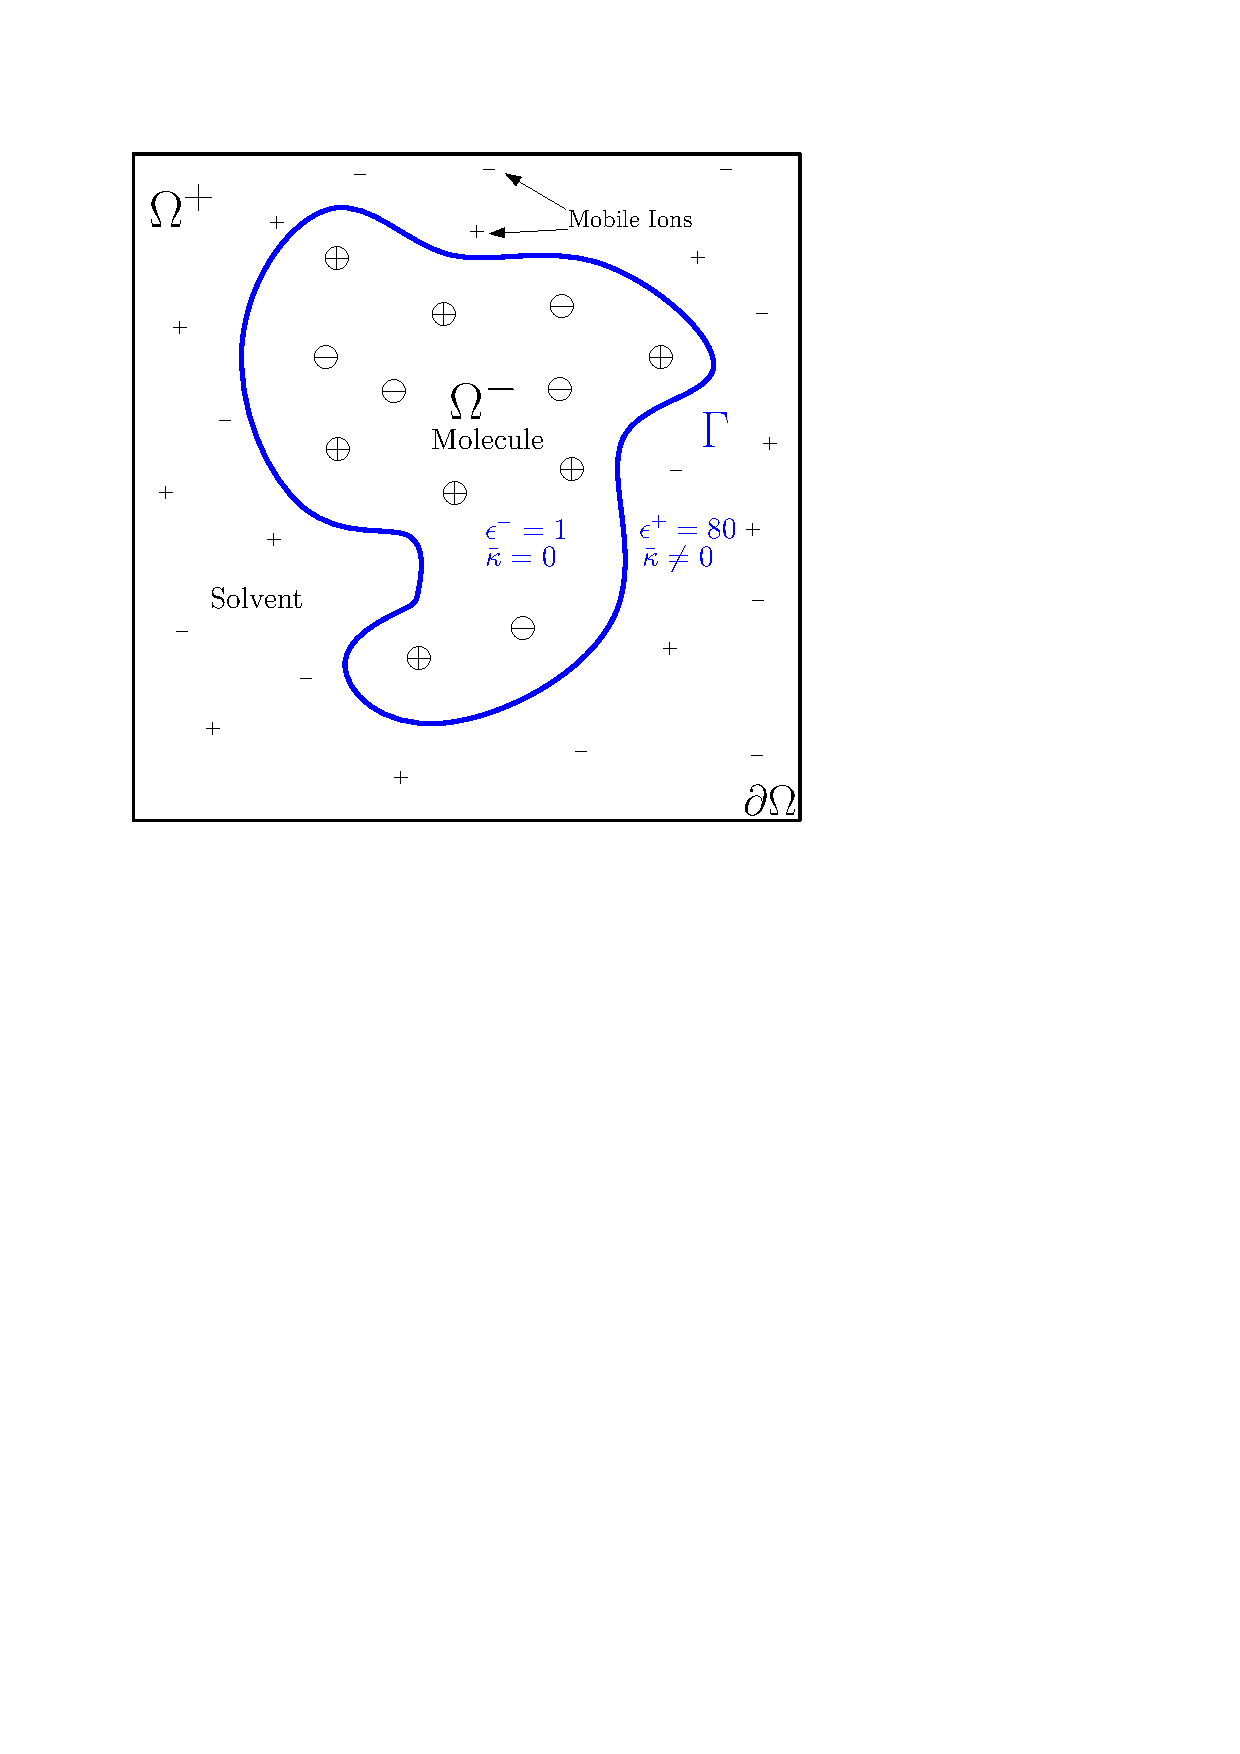
\includegraphics[scale = 0.6]{PBE_domain.pdf}
	\caption{Poisson-Boltzmann Model}
	\label{fig_PBmodel}
\end{figure}

The electrostatic interaction of this solute-solvent system for $\textbf{r} \in \mathbb{R}^3$ is governed by the nonlinear Poisson-Boltzmann Equation (PBE) as, 
\begin{equation}
			-\nabla.(\epsilon(\textbf{r})\nabla \phi(\textbf{r}))+\bar\kappa^2(\textbf{r}) \sinh (\phi(\textbf{r}))=\rho(\textbf{r})\label{pbe} %\\
					%\left[\phi \right]_\Gamma = 0 \textnormal{ and } \left[\epsilon\phi_n\right]_\Gamma = 0 
\end{equation}
with the boundary condition,
\begin{equation}
	\phi_b (\textbf{r}) = \frac{e_c^2}{k_B T} \sum_{i=1}^{N_c} \frac{q_i e^{-|\textbf{r}-\textbf{r}_i | \sqrt{\frac{\bar\kappa^2}{\epsilon^+}} }}{\epsilon^{+}|\textbf{r}-\textbf{r}_i|} \label{bd_cond}
\end{equation}
where the singular source $\rho(\textbf{r})$ term is defined as,
\begin{equation}
	\rho(\textbf{r})= 4\pi \frac{e_c^2}{k_B T}\sum_{i=1}^{N_c} q_i \delta(\textbf{r}-\textbf{r}_i) \label{rho}
\end{equation}
There are two conditions on $\Gamma$ needed to be satisfied from the dielectric theory for the potential $\phi$ and flux density $\epsilon \phi_\textbf{n} $, 
\begin{equation}
\left[\phi \right]_\Gamma = 0 \textnormal{ and } \left[\epsilon\phi_n\right]_\Gamma = 0 \label{ju_cond}
\end{equation}
Here $\textbf{n}=(n_x,n_y,n_z)$ is the outer normal direction on the interface $\Gamma$ and $\phi_\textbf{n}= \frac{\partial \phi}{\partial\textbf{n}} $ is the directional derivative in \textbf{n}. The notation $[f]_\Gamma = f^+-f^-$ represent the difference of the functional value across the interface $\Gamma$.The dielectric constant $\epsilon$ is piecewise such that, $\epsilon(\textbf{r})=\epsilon^-$ for $\textbf{r} \in \Omega^-$ and $\epsilon(\textbf{r})=\epsilon^+$ for $\textbf{r} \in \Omega^+$. Here $N_c$ is the total number of atoms in the solute molecule, $k_B$ is the Boltzmann constant, $e_c$ is the fundamental charge and $q_i$, in the same unit as $e_c$ is the partial charge on the \textit{i}th atom of the solute molecule located at position $\textbf{r}_j$. The Debey-Huckel parameter $\bar\kappa^2 =\Big(\frac{2N_A e_c^2}{100 k_b T}\Big)I_s =  8.486902807$\AA$^{-2} I_s$ from \cite{Holst:1993} for $\textbf{r} \in \Omega^-$ and $\bar\kappa=0$ for $\textbf{r} \in \Omega^+$. Here $N_A$ is Avogadro’s Number and $I_s$ is the molar ionic strength. We have converted the dimensionless electrostatic potential $u$ to the units kcal/mol/$e_c$ at the room temperature $T$ by multiplying it by $0.592183$ as in \cite{Holst:1993}. 

%The reader can refer to REF1 and REF2 for more details about definitions and units of these coefficients. 

%%%%%%%%%%%%%%%%%%%%%%%%%%%%%%%%%%%%%%%%%%%%%%%%%%%%%%%%%%%%%%%%%%%%%%%%%%%%%
\section{ADI Method for pseudo transient PBE}

Using pseudo transient PBE introducing a pseudo-transient variation has become popular approach for solving the nonlinear PB equation \cite{Sayyed-Ahmad2004, Shestakov2002, zhao_pseudo-time-coupled_2011, zhao_operator_2014}. In this approach equation (\ref{pbe}) is converted to the following time dependent PBE (TPBE),

\begin{equation}
			\frac{\partial \phi}{\partial t}(\textbf{r},t)=\nabla.(\epsilon(\textbf{r})\nabla \phi(\textbf{r},t))-\bar\kappa^2(\textbf{r}) \sinh (\phi(\textbf{r},t))+\rho(\textbf{r})\label{tpbe} %\\
					%\left[\phi \right]_\Gamma = 0 \textnormal{ and } \left[\epsilon\phi_n\right]_\Gamma = 0 
\end{equation}
%In \cite{geng_fully_2013} equation (\ref{tpbe}) has later been separated in two separate equation using a first order time splitting like equation (\ref{non_linear_ADI}) and (\ref{diffusion_ADI}) in section \ref{sec:GFM-ADI}. Then the nonlinear equation has been solved by an analytical solution and the Douglas-Rachford ADI scheme has been used for the other diffusion equation. But in terms of intrer
In \cite{geng_fully_2013} equation (\ref{tpbe}) has later been separated in two separate equation using a first order time splitting like the following equations, 
\begin{eqnarray}
  \frac{\partial w}{\partial t}&=& -\bar\kappa^2 \sinh(w) \text{ with } W^n=\phi^n\text{ and } t \in \left[t_n,t_{n+1}\right]\label{eq_nonl_ADI1}\\
 \frac{\partial v}{\partial t}&=&  \nabla . (\epsilon\nabla v) \text{ with } V^n=W^{n+1}\text{ and } t \in \left[t_n,t_{n+1}\right]	 \label{eq_diff_ADI1}
\end{eqnarray}  

Where $V^{n+1} = \phi^{n+1}$. After using an analytical solution for equation (\ref{eq_nonl_ADI1}) a Douglas-Rachford type ADI scheme has been introduced in \cite{geng_fully_2013}. The discretization of equation (\ref{eq_diff_ADI1}) using backward-Euler integration in time and central differencing in space results in, 
\begin{eqnarray}
	v_{i,j,k}^{n+1} &=v_{i,j,k}^{n}+\Delta t \left(\delta_x^2+\delta_y^2+\delta_z^2\right)v_{i,j,k}^{n+1}+\Delta t \rho({\bf r}) \label{imp-eu}
\end{eqnarray}

%{\color{red} Should I include the equations here?}
Where $\delta_x,\delta_y$ and $\delta_z$ are the central finite difference operators in $x,y$ and $z$ directions as, 
  \begin{eqnarray}
 \begin{aligned}
	\delta_x^2\left(v_{i,j,k}^n\right)&= \frac{1}{h^2} \left(\epsilon_{i+\frac{1}{2},j,k}(v_{i+1,j,k}^n-v_{i,j,k}^n)+\epsilon_{i-\frac{1}{2},j,k}(v_{i-1,j,k}^n-v_{i,j,k}^n)\right) \\ \label{dif_opx_adi1}
	\delta_y^2\left(v_{i,j,k}^n\right)&= \frac{1}{h^2} \left(\epsilon_{i,j+\frac{1}{2},k}(v_{i,j+1,k}^n-v_{i,j,k}^n)+\epsilon_{i,j-\frac{1}{2},k}(v_{i,j-1,k}^n-v_{i,j,k}^n)\right) \\ %\label{dif_opy}
	\delta_z^2\left(v_{i,j,k}^n\right)&=\frac{1}{h^2} \left(\epsilon_{i,j,k+\frac{1}{2}}(v_{i,j,k+1}^n-v_{i,j,k}^n)+\epsilon_{i,j,k-\frac{1}{2}}(v_{i,j,k-1}^n-v_{i,j,k}^n)\right)  
	\end{aligned}
\end{eqnarray}
Here the $\epsilon$-halfs ($\epsilon_{i+\frac{1}{2},j,k},\epsilon_{i,j+\frac{1}{2},k}$ and $\epsilon_{i,j,k+\frac{1}{2}}$) are the average of the dielectric constants value at two adjacent grid point in $x,y$ and $z$ directions. Then the following Douglas-Rachford ADI scheme has been used in \cite{geng_fully_2013}
   
\begin{eqnarray}
%\begin{aligned}
		\left(1- \Delta t \delta_x^2\right)v_{i,j,k}^{*}&=&\left[1+ \Delta t \left(\delta_y^2+\delta_z^2 \right)\right]v_{i,j,k}^{n}+\Delta t \rho({\bf r})\label{eq_ADI1}\nonumber \\ 
		\left(1-\Delta t \delta_y^2\right)v_{i,j,k}^{**}&=&v_{i,j,k}^{*}- \Delta t \delta_y^2\left(v_{i,j,k}^{n}\right)\label{GFM-ADI2}\\
		\left(1- \Delta t \delta_z^2\right)v_{i,j,k}^{n+1}&=&v_{i,j,k}^{**}- \Delta t \delta_z^2\left(v_{i,j,k}^{n}\right)\label{GFM-ADI3}\nonumber
%\end{aligned}		\label{1dadi}
\end{eqnarray} 

The ADI methods discussed in \cite{geng_fully_2013} are promising tool to solve the nonlinear PBE but it is not focused on the issues due to the singularity at the source terms and the jump conditions on the interface. As we observed in the chapter \ref{chap:num_vald}, these two issues reduced the accuracy and stability of the ADI method significantly.  
       
%%%%%%%%%%%%%%%%%%%%%%%%%%%%%%%%%%%%%%%%%%%%%%%%%%%%%%%%%%%%%%%%%%%%%%%%%%%%%


\section{Cleaning ADI-MSMS package to develop REG-GFM-MSMS package}	
To simulate the ADI Methods in \cite{geng_fully_2013} and the LOD Methods in \cite{Wilson2016}, Professor Shan Zhao, Dr. Weihua Geng form the Southern Methodists University and Leighton Wilson developed a coding package named ADI-MSMS. This package uses two types of protein data files for a particular protein as inputs and calculated the electrostatic potential $\phi$ and the solvation energy as the outputs. The input files were generated from the {\it .pdb} and {\it .pqr } file. This package used the following two sub-packages developed by others,

\begin{itemize}
	\item {\bf FISHPACK90:} This sub-package was originally developed by the NCAR (National Center for Atmospheric Research) back in the late 70's and revised later in 90's. It is a collection of FORTRAN programs and subroutines that solves second- and fourth-order finite difference approximations to  the elliptic Partial Differential Equations (PDEs). In ADI-MSMS package its been used to the solve the Poisson Equation for a special case of the PBE when the protein molecule is considered to be in vacuum instead of surrounded by the solvent.
	\item {\bf MSMS:} It is a program \cite{MSMS} written in the programming language C to compute the molecular surface. It was developed by  Michel Sanner and his team  at the Molecular Graphics Laboratory (TSRI). It uses the input files for the ADI-MSMS package and produces two files with extensions {\it .vert} and {\it .face}. Later these output files from the MSMS package are used to decide whether a grid point is inside or outside or on the molecular interface. 
\end{itemize} 

%	{\bf INPUT}: File Type 1 containing the    


\begin{figure}[!ht]
	\centering
	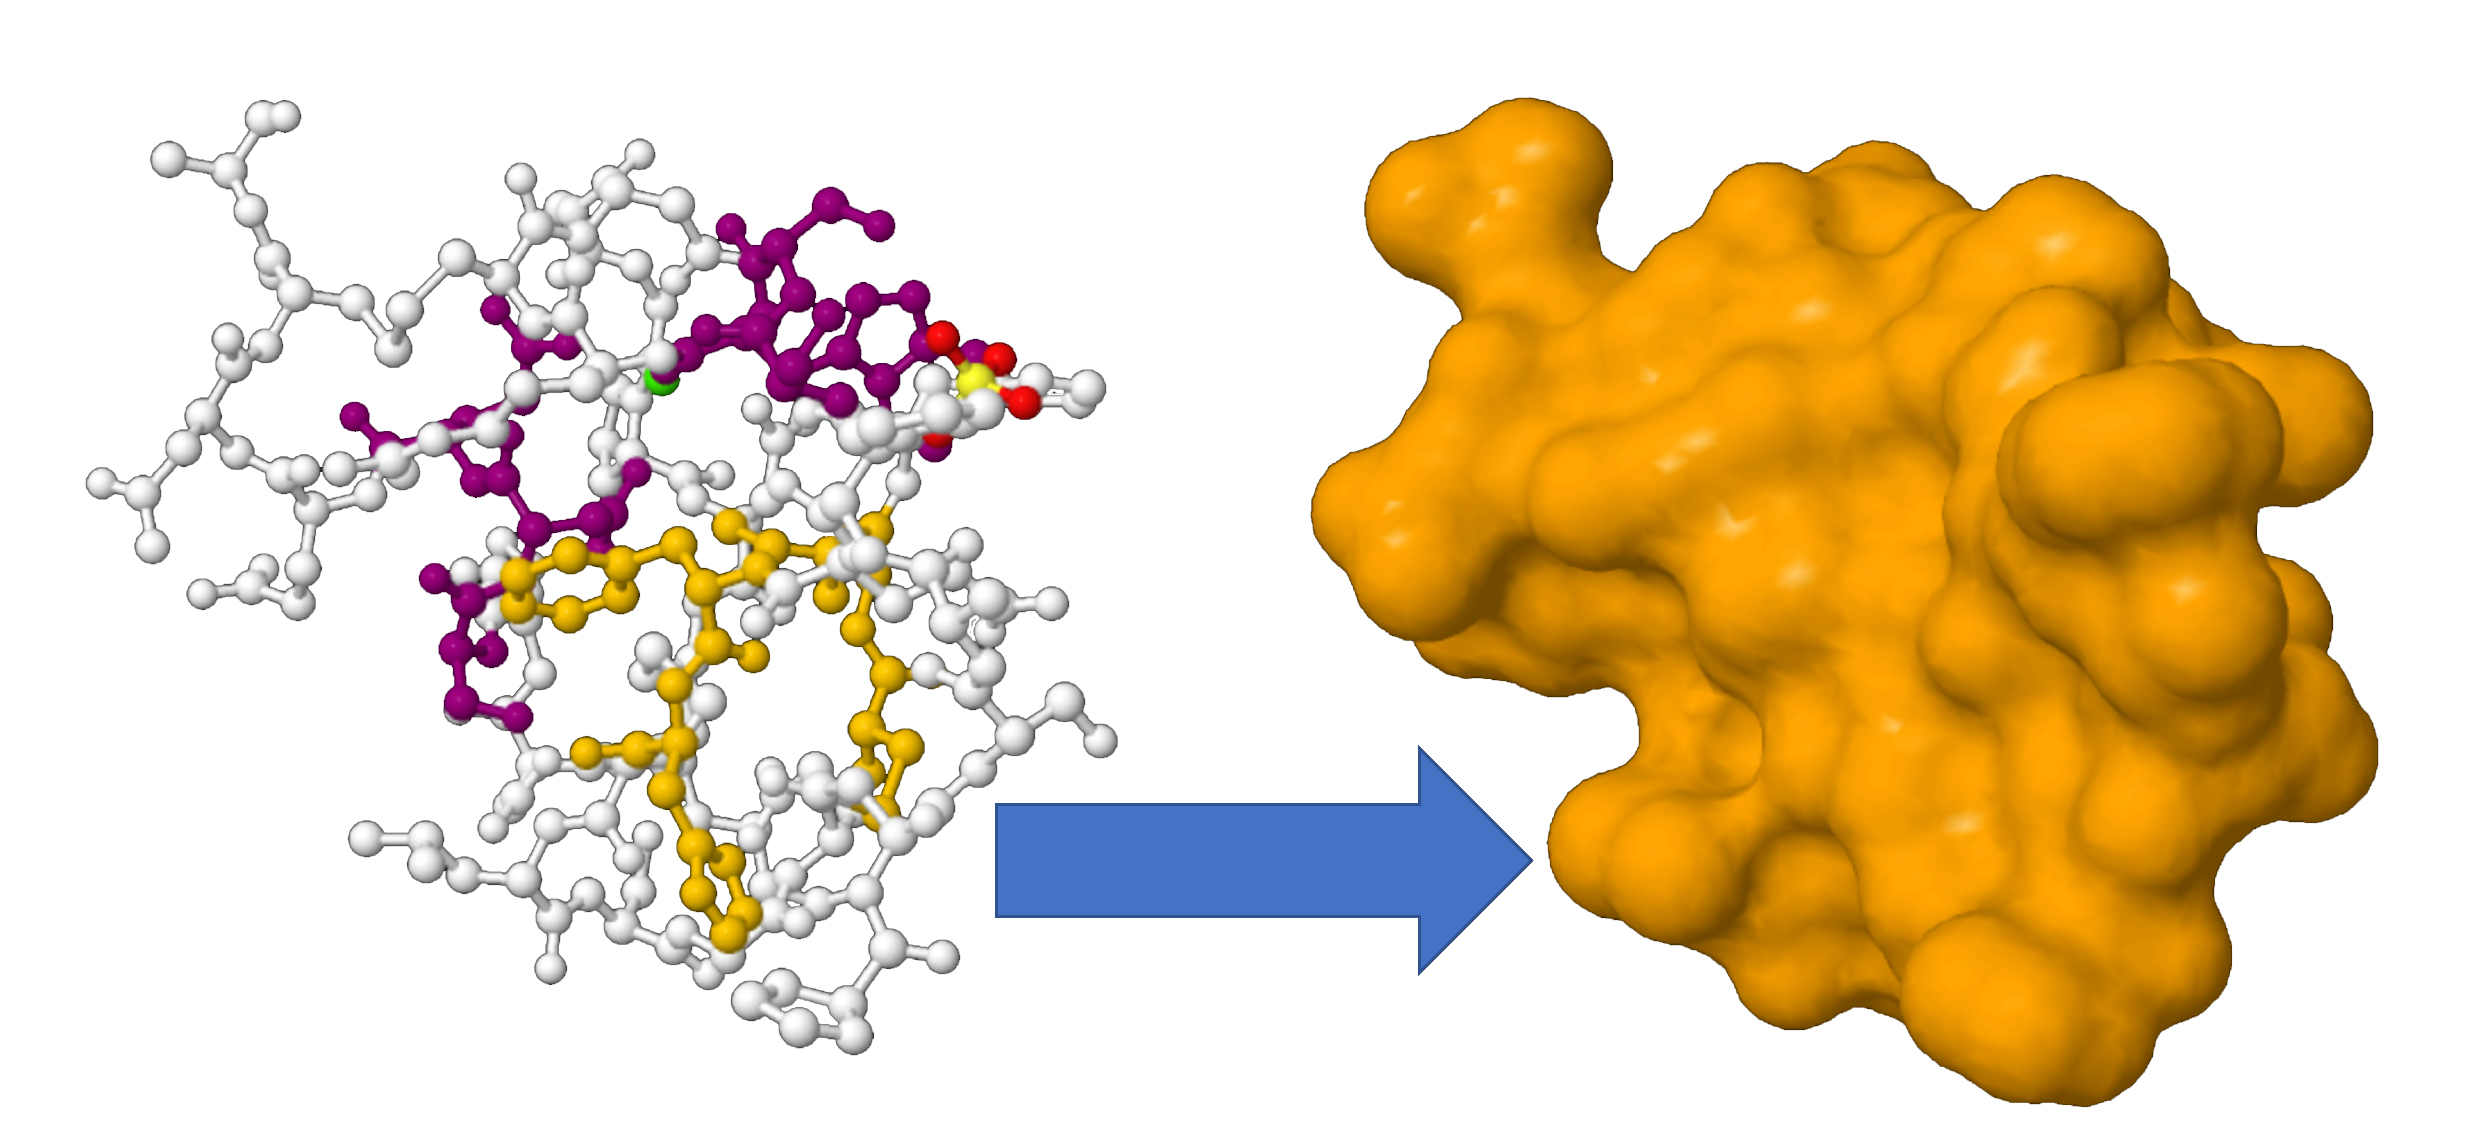
\includegraphics[scale  = .35]{1ajj_surface_white.jpg}	
	\caption{Molecular Surface of the protein \textit{1ajj} generated by MSMS}
\end{figure}

%Then this ADI-MSMS package followed the following steps.
%\begin{enumerate}
%	\item Reading $x,y,z$ coordinates, radius and atomic charges from the input files.
%	\item Distributing the atomic charges to the nearest grid points as partial charges. 
%	\item   
%\end{enumerate}
Though this ADI-MSMS package served well for the previous works for the ADI and LOD methods, it was time to do a major revision. When we started with this ADI-MSMS package we had to fix the following issues to prepare it to replace the Numerical methods by our proposed methods to solve the PBE,

\begin{itemize}
	\item FISHPACK90 got updated a long time ago and it was failing to comply with the new FORTRAN compilers. Also the subsidiary FFT(Fast Fourier Transform) routines were passing arguments of one type and using them as another. So we made the following adjustments.
		\begin{enumerate}
			\item In the subroutine {\it POISOLVE3D} the variables {\it BDXS, BDXF, BDYS, BDYF, BDZS, BDZF} were declared as real variables but used later as two dimensional arrays. We fixed this issues by declaring them in proper dimension and size.
			\item The variable {\it IFAC} was declared as integer but it was meant to be a real variable.
			\item In the module {\it fish} the arrays {\it rew} and {\it cxw} were declared as pointers but this type of declarations became obsolete for the new FORTRAN compilers. We updated them to be declared as allocatable.  
		\end{enumerate}
	\item Using two different type of files as inputs for the ADI-MSMS package was requiring an extra manual step outside the package to prepare the protein data to be usable. We updated the subroutine {\it readin} to read the necessary data directly from the {\it .pqr} file. It was a more user friendly process and better in terms of data management for the whole package.
	\item Unlike the ADI or LOD methods we needed the exact location of the points where the molecular surface was intersecting with the gridlines. We had to add extra features in the package to extract that information from the output files produced by the MSMS package.     
\end{itemize}  

After cleaning the bugs form ADI-MSMS and adding the new features we developed a new coding package REG-GFM-MSMS to incorporate all three of our proposed numerical methods to solve the PBE. 


